\chapter{Blinn-Phong Lighting}
\label{chap:BlinnPhong}

In this chapter we add lighting to the scene we previously set up.
We first implement the Blinn-Phong lighting model.
After that, we refine its behavior adding materials to our objects and lights.

\section{Vulkan Related Details}

Before starting to implement the lighting model, we must clarify some technical
things related to Vulkan.

\subsection{Pipeline State Objects}

The scene's entities can be divided into two groups: the entities to which we
apply lighting, i.e. the floor and the cube; and the entities to which we
don't apply lighting, i.e. the light source itself.
This means that we must use two sets of shaders: one that implements
the Blinn-Phong lighting model, and the other that simply draws a flat color.
For this reason, we need to create two different pipeline state objects.

\subsection{Updating Our Vertex Data}

For each fragment, the lighting model needs to know the surface normal.
To solve this problem, we store, for each vertex, a normal vector.
Here we can see a visualization of the quad and cube vertex normals.

\begin{figure}[H]
    \centering
    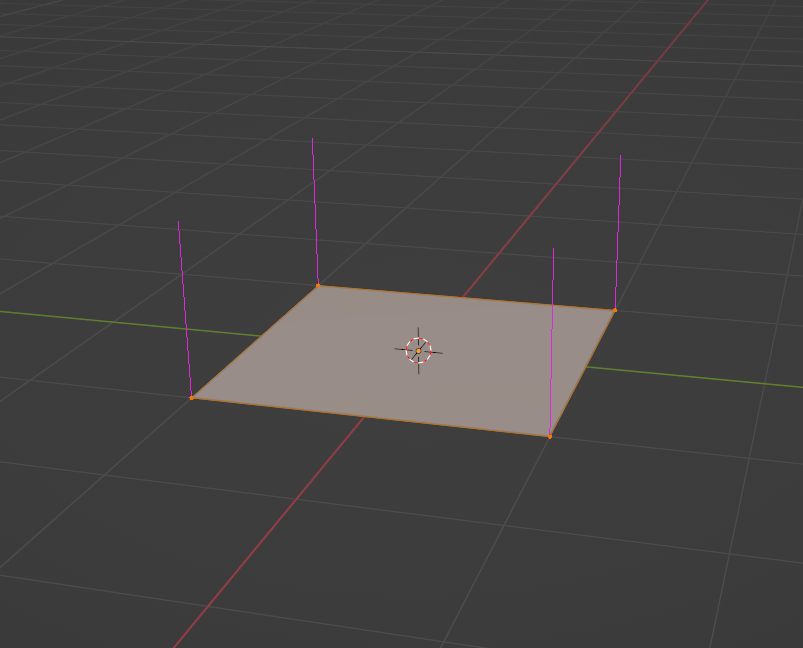
\includegraphics[scale=0.40]{images/ChBlinnPhong/QuadVertexNormals.png}
    \caption{Quad vertex normals visualization}
    \label{fig::QuadVertexNormals}
\end{figure}

\begin{figure}[H]
    \centering
    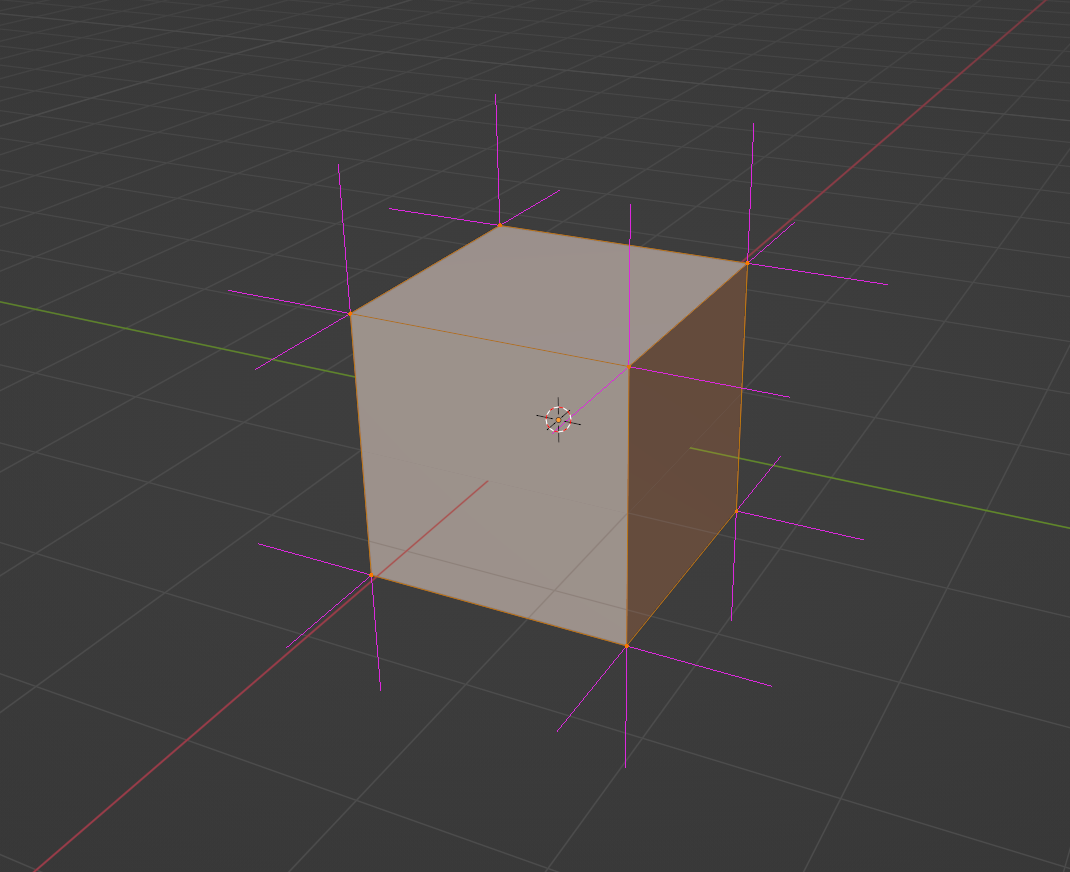
\includegraphics[scale=0.30]{images/ChBlinnPhong/CubeVertexNormals.png}
    \caption{Cube vertex normals visualization}
    \label{fig::CubeVertexNormals}
\end{figure}

\section{Blinn-Phong Lighting Model}

In computer graphics, we approximate lighting using simplified models.
The lighting model we implement here is called Blinn-Phong.
This model divides light into three components: ambient light, diffuse light and
specular light.

\subsection{Ambient Lighting}

In the real world, even when there is no apparent light source,
objects aren't completely dark.
This is because light can come from different sources around us, even if
they are not directly visible.
Indeed, light scatters and bounces in different directions.
Thus, some light sources can indirectly light our objects.
To simulate this light property, we use a small constant light value that we
add to our objects' lighting.

\begin{minipage}{\linewidth}{\noindent}
    \lstinputlisting[
        language=C++,
        caption={Computing ambient component},
        label={lst::ShadeAmbient}
        ]{src/ChBlinnPhong/ShadeAmbient.frag}
\end{minipage}

\begin{figure}[H]
    \centering
    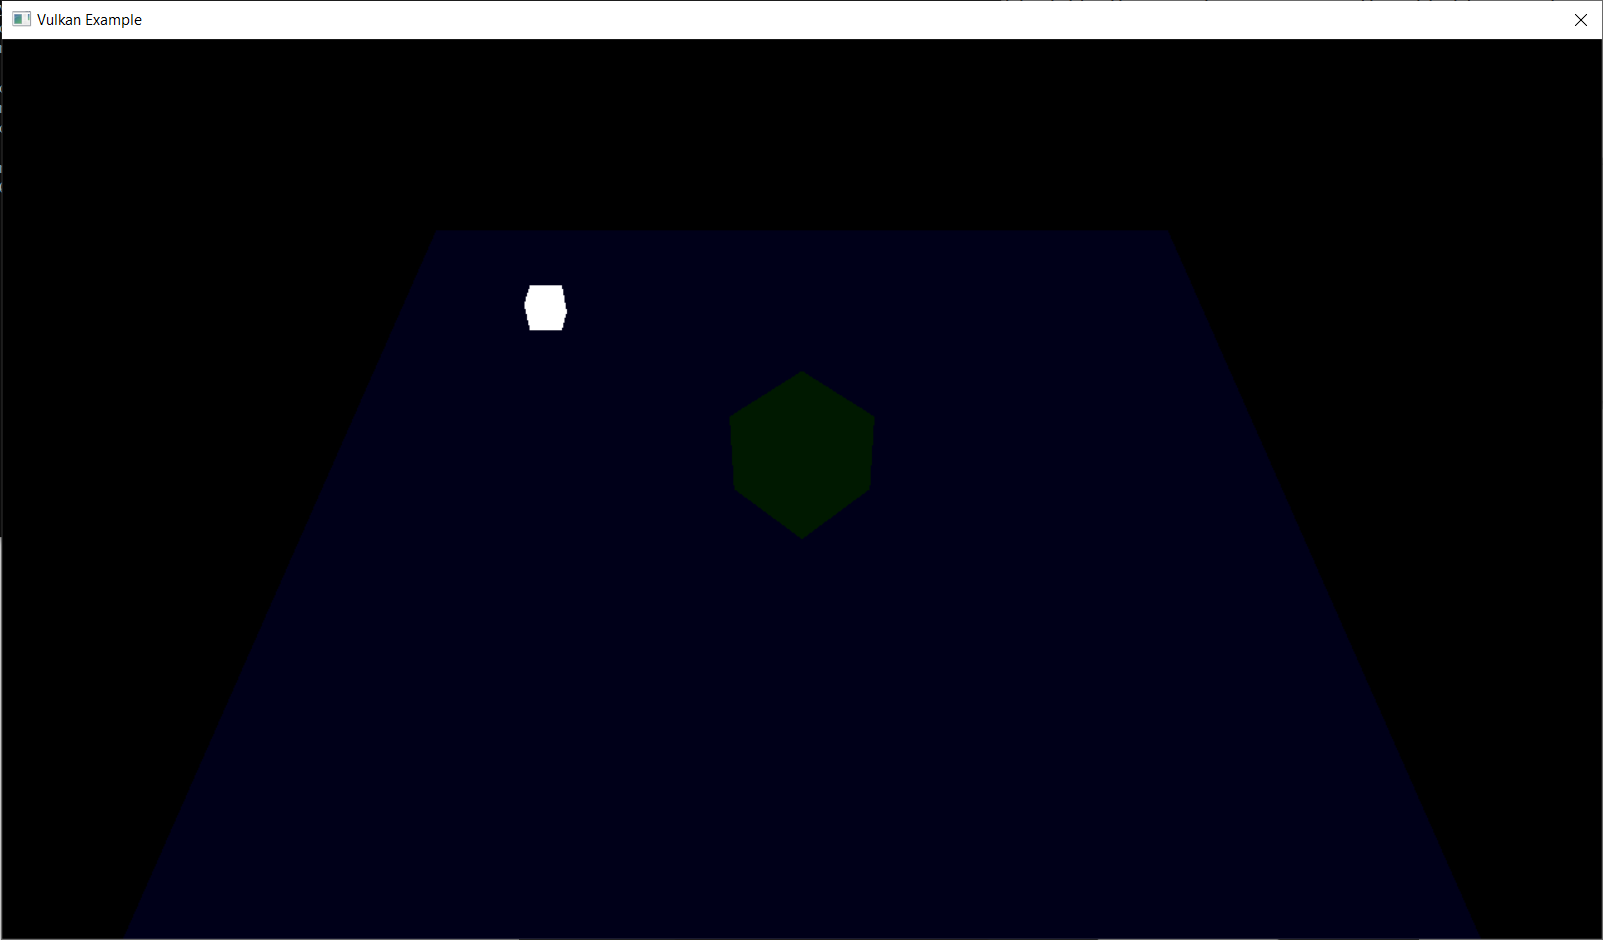
\includegraphics[scale=0.25]{images/ChBlinnPhong/SceneAmbient.png}
    \caption{Scene with ambient lighting}
    \label{fig::SceneAmbient}
\end{figure}

\subsection{Diffuse Lighting}

Diffuse lighting simulates the impact a light has on an opaque object.
In simple terms, the more a part of the object faces the light, the brighter
it becomes.
The diffuse impact is the strongest when
the angle between the surface's normal and the light ray is zero.
The diffuse impact will be zero when the angle is greater than or equal to
ninety degrees.

\begin{figure}[H]
    \centering
    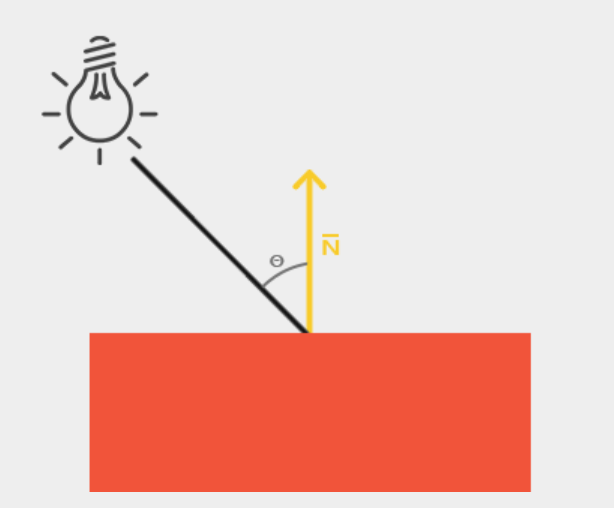
\includegraphics[scale=0.40]{images/ChBlinnPhong/DiffuseLighting.png}
    \caption{Diffuse lighting}
    \label{fig::DiffuseLighting}
\end{figure}

\begin{minipage}{\linewidth}{\noindent}
    \lstinputlisting[
        language=C++,
        caption={Computing diffuse component},
        label={lst::ShadeDiffuse}
        ]{src/ChBlinnPhong/ShadeDiffuse.frag}
\end{minipage}

\begin{figure}[H]
    \centering
    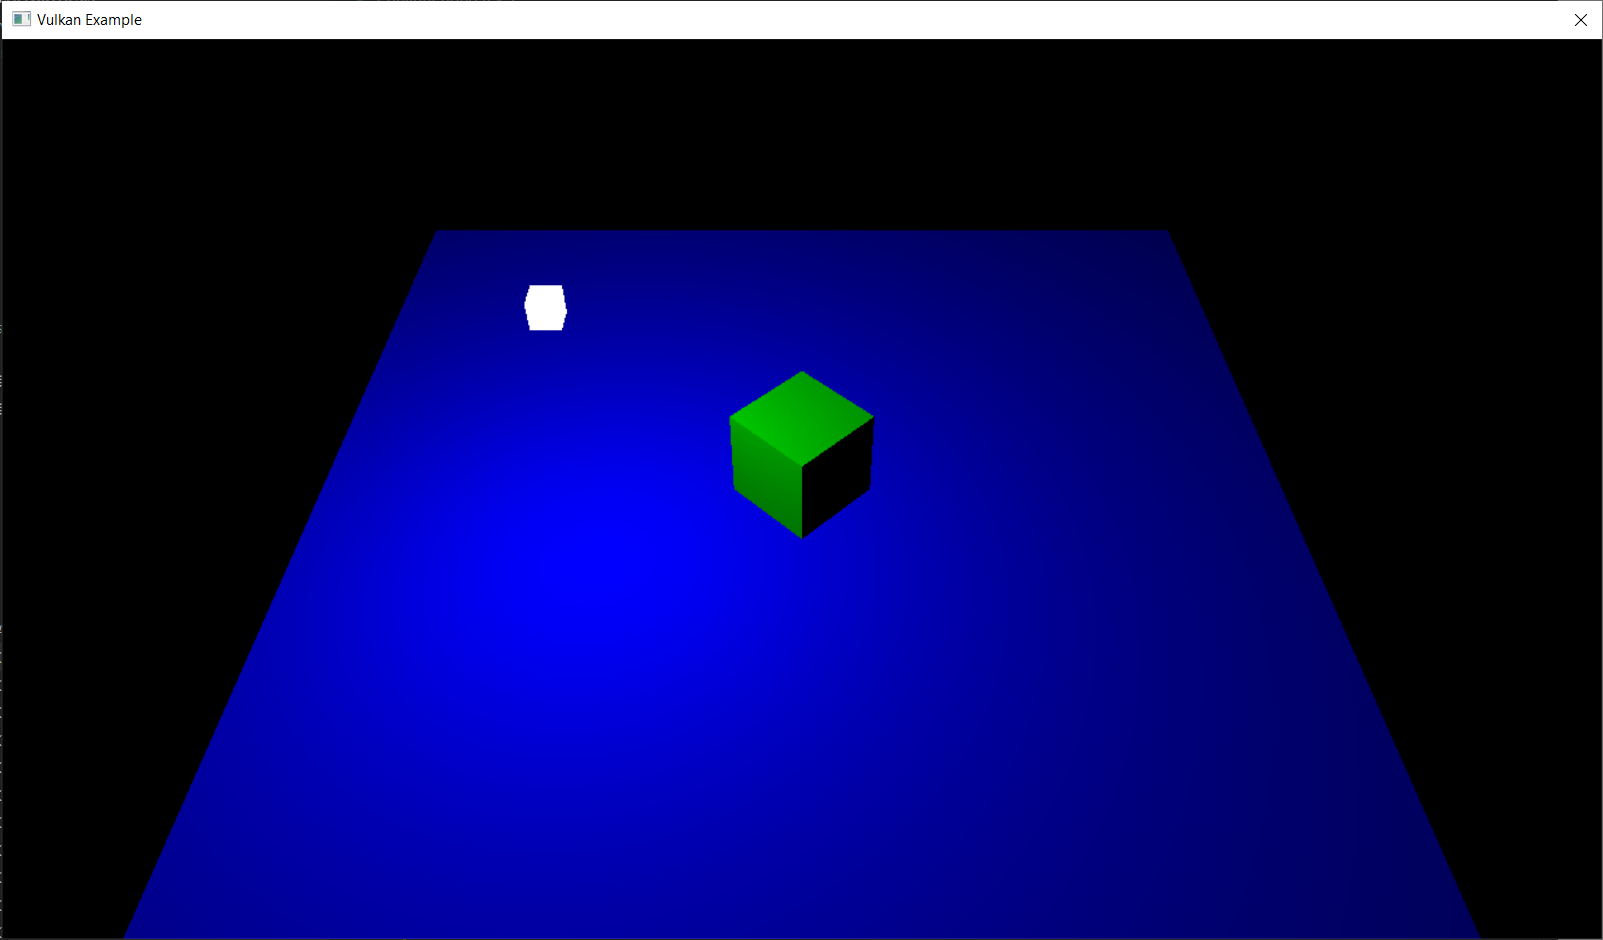
\includegraphics[scale=0.25]{images/ChBlinnPhong/SceneDiffuse.png}
    \caption{Scene with diffuse lighting}
    \label{fig::SceneDiffuse}
\end{figure}

\subsection{Specular Lighting}

Specular lighting simulates the bright spot that lights cause on shiny objects.
This spot is called specular highlight.
The specular impact is the strongest when our view direction is perfectly
aligned with the light ray that is reflected off the object's surface.
The more our view deviates form the reflected vector, the less the specular
impact will be.

To compute the specular impact we first compute a unit vector exactly
halfway between the view direction and the light direction.
The closer this halfway vector aligns with the surface's normal, the higher
the specular impact.

\begin{figure}[H]
    \centering
    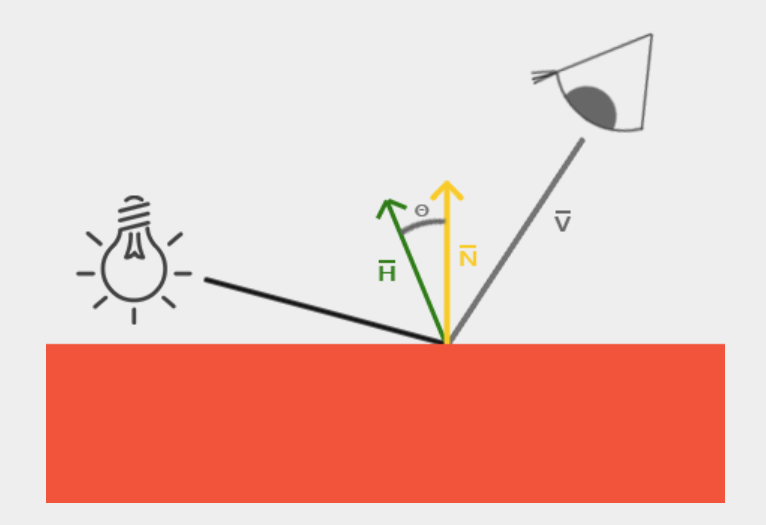
\includegraphics[scale=0.40]{images/ChBlinnPhong/SpecularLighting.png}
    \caption{Specular lighting}
    \label{fig::SpecularLighting}
\end{figure}

\begin{minipage}{\linewidth}{\noindent}
    \lstinputlisting[
        language=C++,
        caption={Computing specular component},
        label={lst::ShadeSpecular}
        ]{src/ChBlinnPhong/ShadeSpecular.frag}
\end{minipage}

\begin{figure}[H]
    \centering
    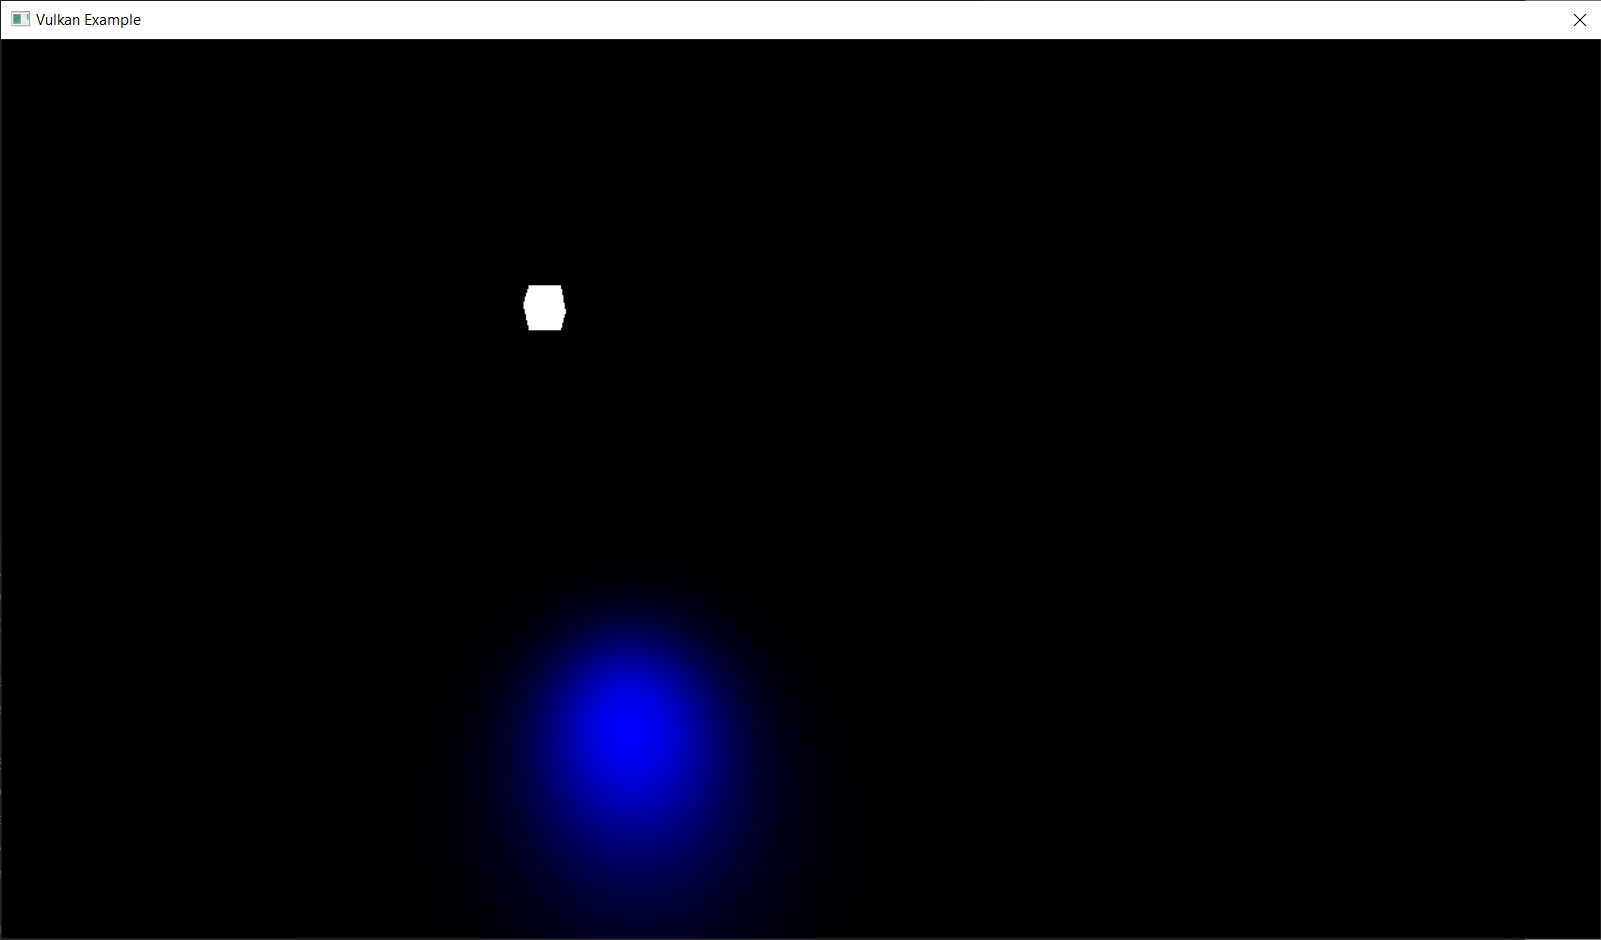
\includegraphics[scale=0.25]{images/ChBlinnPhong/SceneSpecular.png}
    \caption{Scene with specular lighting}
    \label{fig::SceneSpecular}
\end{figure}

\subsection{Putting It All Together}

Finally we can merge ambient, diffuse and specular components together.
We do this by simply adding them together.

\begin{minipage}{\linewidth}{\noindent}
    \lstinputlisting[
        language=C++,
        caption={Computing final light value},
        label={lst::ShaderMergeComponents}
        ]{src/ChBlinnPhong/ShaderMergeComponents.frag}
\end{minipage}

\begin{figure}[H]
    \centering
    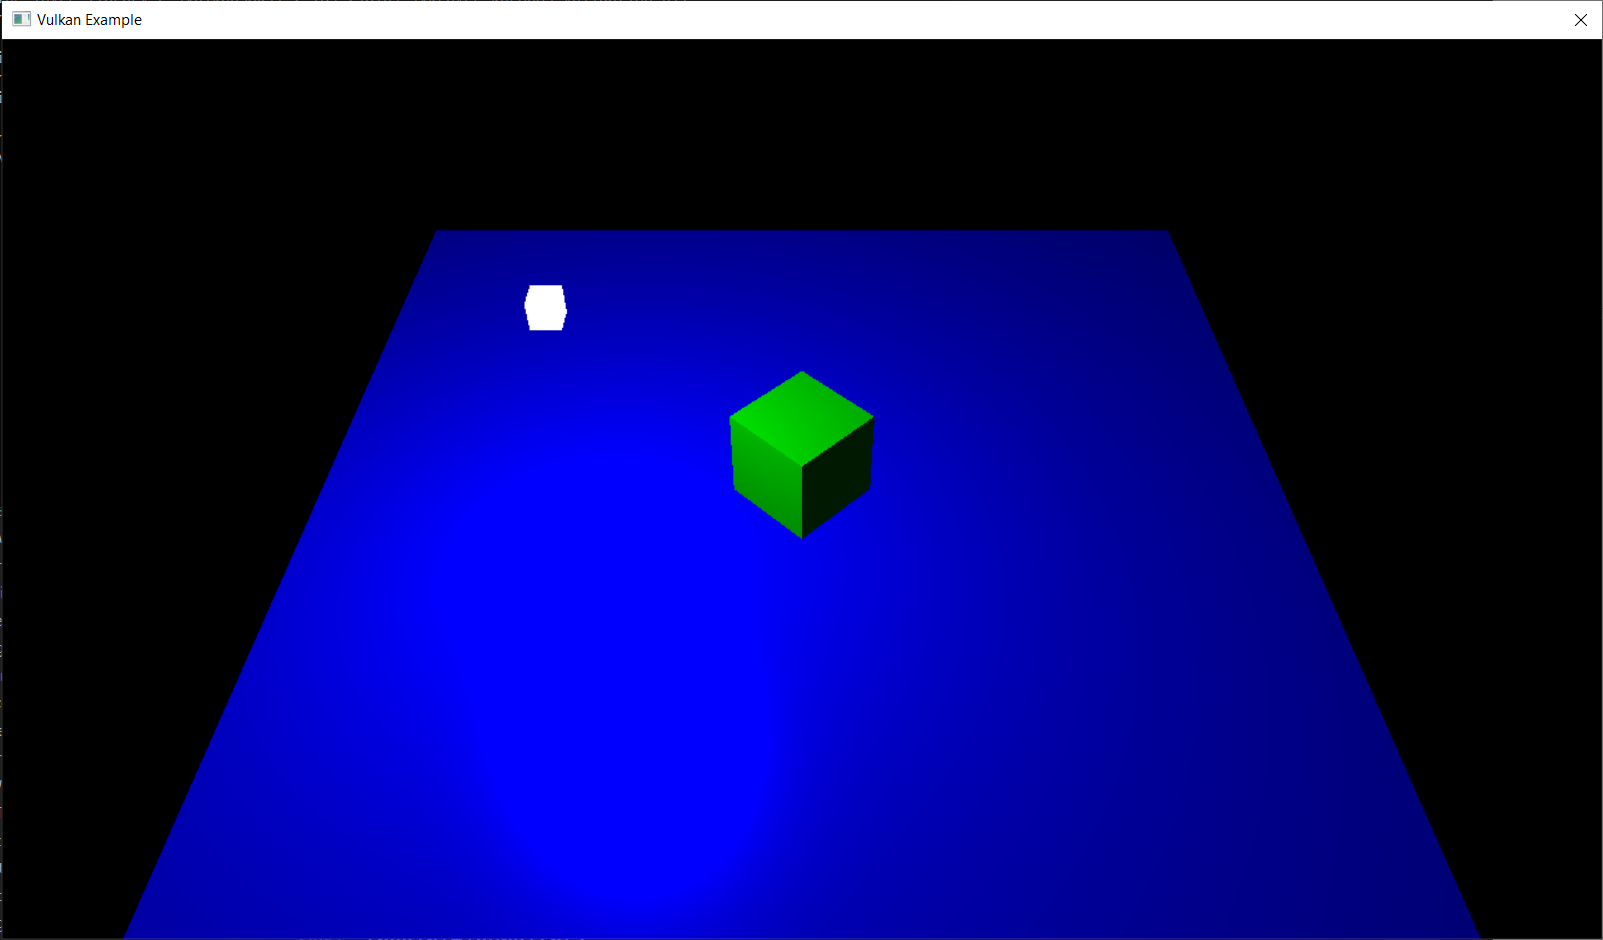
\includegraphics[scale=0.25]{images/ChBlinnPhong/SceneLit.png}
    \caption{Scene with ambient, diffuse and specular lighting}
    \label{fig::SceneLit}
\end{figure}

\section{Materials}

Real world objects have different reactions to light.
We simulate this property using materials.
We can describe a material by specifying four different properties:
one for each lighting component plus a shininess value.
We can simulate a lot of different real world materials simply using
different combinations of these four values.

\subsection{Scene Materials}

In our scene, we use two materials.
The \texttt{turquoise} material is used by the floor entity.
The \texttt{emerald} material is used by the cube entity.

\begin{minipage}{\linewidth}{\noindent}
    \lstinputlisting[
        language=C++,
        caption={Materials used in our scene},
        label={lst::Materials}
        ]{src/ChBlinnPhong/Materials.cpp}
\end{minipage}

\subsection{Blinn-Phong With Object Materials}

The ambient material property defines what color the surface reflects
under ambient lighting.
This is usually the same as the surface's color.
The diffuse material property defines the color of the surface under
diffuse lighting.
The specular material property defines the color of the specular highlight.
The shininess material property affects the specular highlight's radius.

\begin{minipage}{\linewidth}{\noindent}
    \lstinputlisting[
        language=C++,
        caption={Blinn-Phong lighting using object materials},
        label={lst::ShadeMaterials}
        ]{src/ChBlinnPhong/ShadeMaterials.frag}
\end{minipage}

\begin{figure}[H]
    \centering
    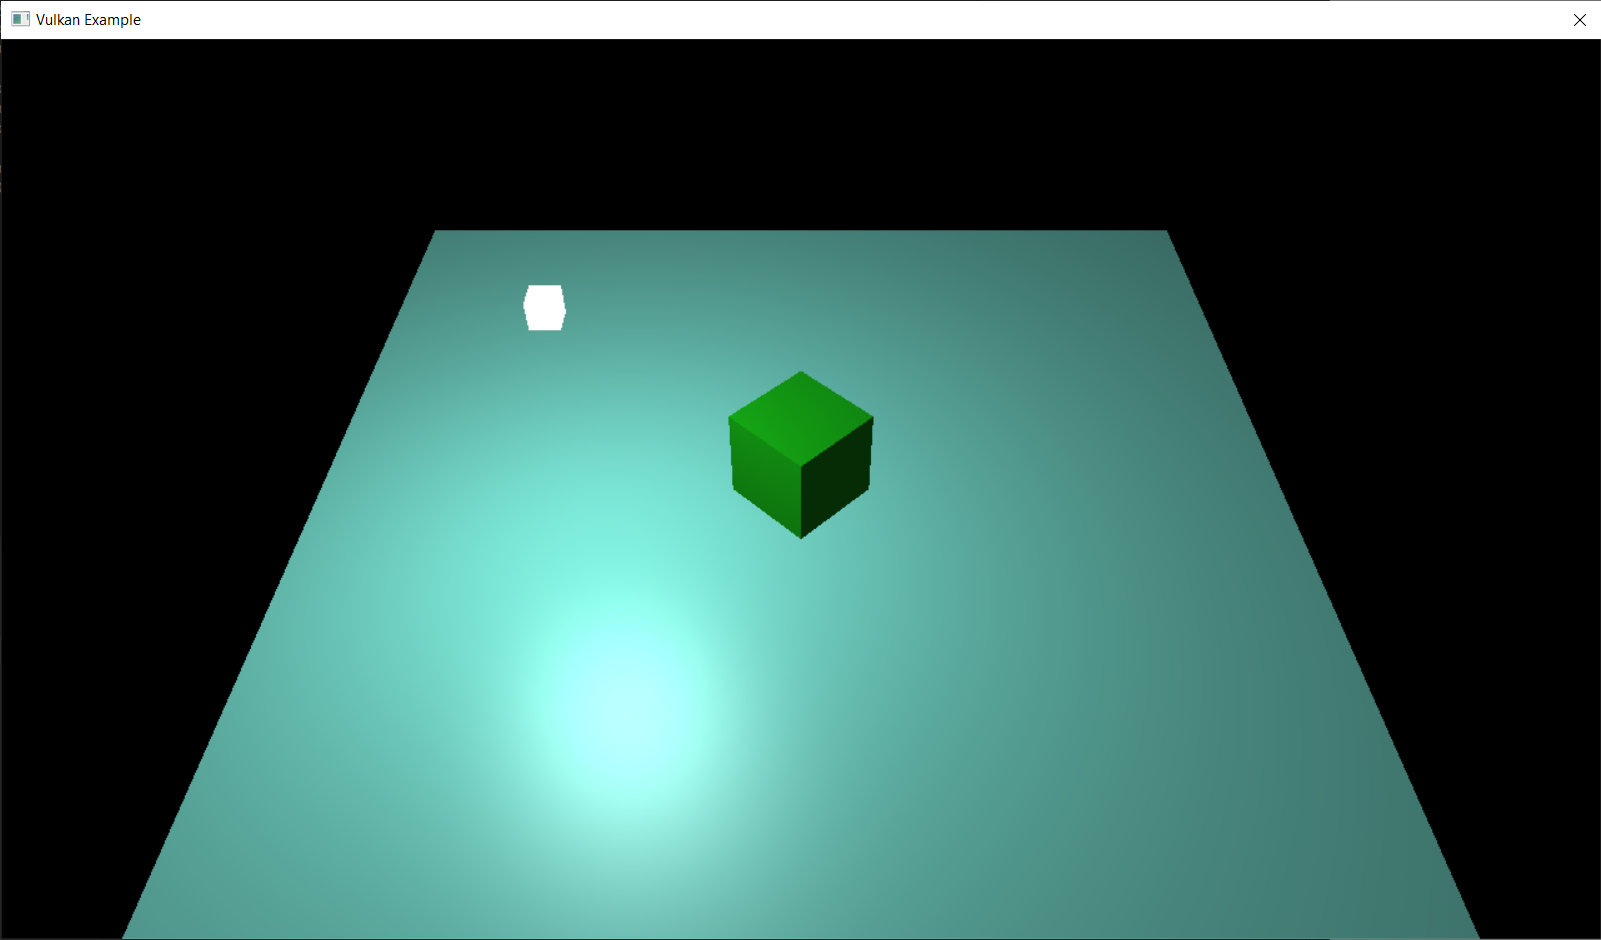
\includegraphics[scale=0.25]{images/ChBlinnPhong/SceneMaterials.png}
    \caption{Scene lighting using material properties}
    \label{fig::SceneMaterials}
\end{figure}

\subsection{Blinn-Phong With Object And Light Materials}

In the previous image, we see that the objects are too bright.
This is due to the fact that the ambient, diffuse and specular
colors are computed simply using the light's color.
Lights also have different intensities for their ambient,
diffuse and specular components.

We set the ambient component to a low intensity because we don't want the
ambient color to be too dominant.
We set the diffuse component to a slightly darkened version of the light's
color.
We set the specular component to the light's color, shining at full intensity.

\begin{minipage}{\linewidth}{\noindent}
    \lstinputlisting[
        language=C++,
        caption={Our scene light's material},
        label={lst::LightMaterial}
        ]{src/ChBlinnPhong/LightMaterial.cpp}
\end{minipage}

\begin{minipage}{\linewidth}{\noindent}
    \lstinputlisting[
        language=C++,
        caption={Blinn-Phong lighting using object and light materials},
        label={lst::ShadeLightMaterial}
        ]{src/ChBlinnPhong/ShadeLightMaterial.frag}
\end{minipage}

\begin{figure}[H]
    \centering
    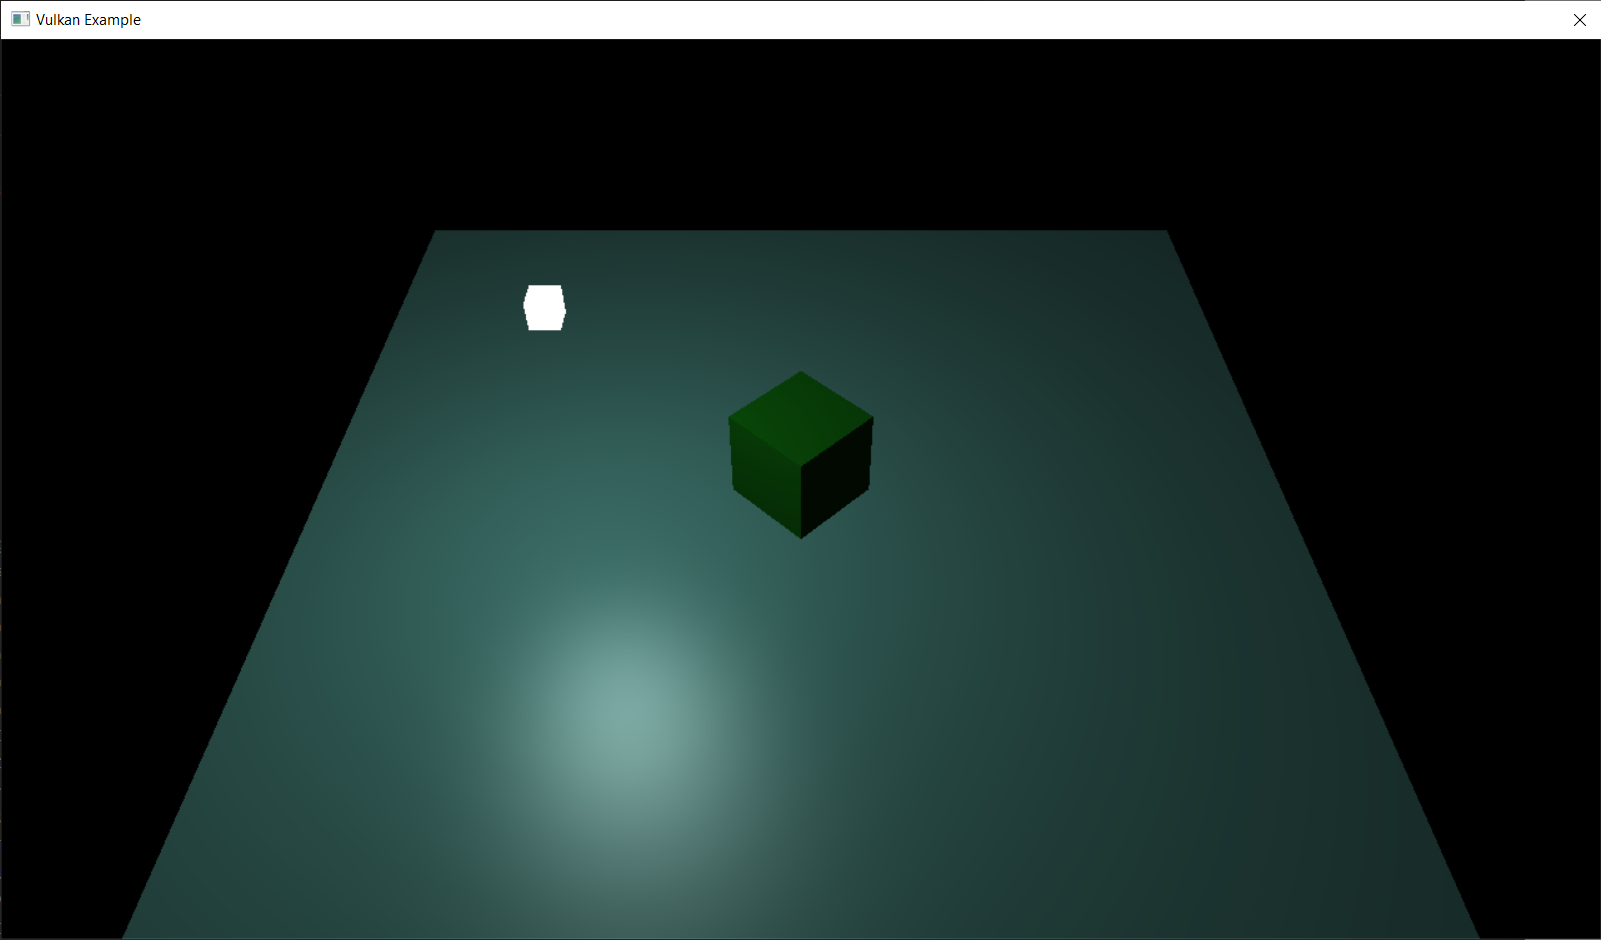
\includegraphics[scale=0.25]{images/ChBlinnPhong/SceneMaterialsLight.png}
    \caption{Scene lighting using object and light materials}
    \label{fig::SceneMaterialsLight}
\end{figure}
